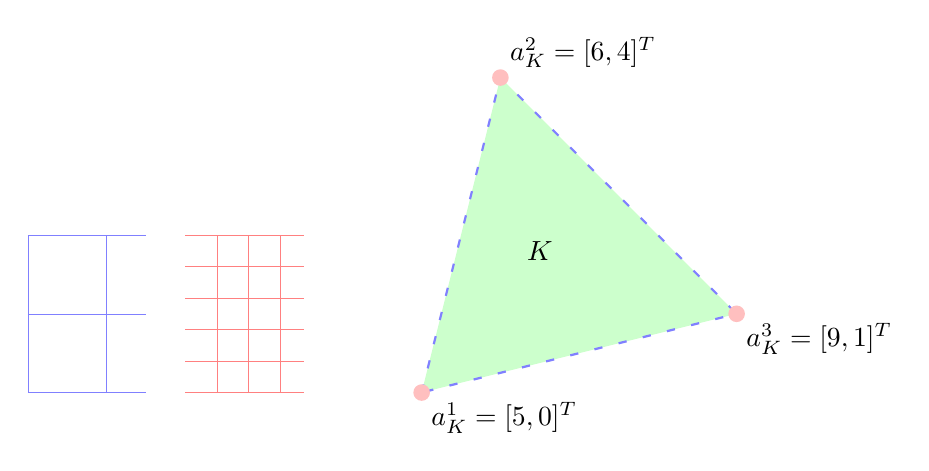
\begin{tikzpicture}
	[Karl's grid/.style={help lines,color=#1!50},Karl's grid/.default=blue]
	\draw[Karl's grid] (0,0) grid (1.5,2);
	\draw[step=0.4,Karl's grid=red] (2,0) grid (3.5,2);	
	\filldraw[fill=green!20,draw=blue!50]
		 [loosely dashed, thick] (5,0)--(6,4)--(9,1) --cycle;
	\fill[pink] (5,0) circle (3pt)  (6,4) circle (3pt)  (9,1) circle (3pt);
	\node[anchor=north west] at (5,0) {$a_K^1=[5,0]^T$};
	\node[anchor=south west] at (6,4) {$a_K^2=[6,4]^T$};
	\node[anchor=north west] at (9,1) {$a_K^3=[9,1]^T$};
	\node at (6.5,1.8) {$K$};
\end{tikzpicture}	
	
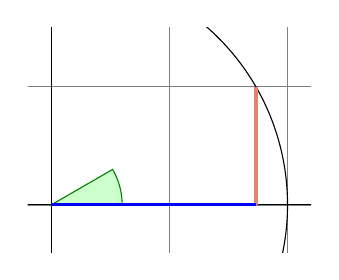
\begin{tikzpicture}[scale=3]
	\clip(-0.1,-0.2)rectangle(1.1,0.75);
	\draw[step=.5cm,gray,very thin] (-1.4,-1.4)grid(1.4,1.4);
	\draw(-1.5,0)-- (1.5,0);
	\draw(0,-1.5)--(0,1.5);
	\draw(0,0)circle[radius=1cm];
	\filldraw[fill=green!20,draw=green!50!black](0,0)-- (3mm,0mm)
	 	arc[start angle=0,end angle=30,radius=3mm]--cycle;
	\draw[red!80!green!60, very thick]  (30:1cm)-- ++(0,-0.5);
	\draw[blue,very thick] (30:1cm) +(0,-0.5)-- (0,0);
\end{tikzpicture}
	
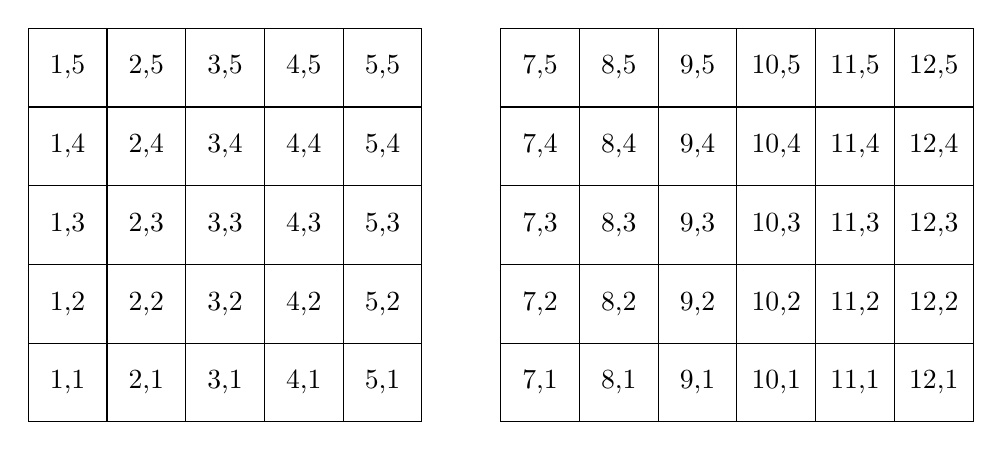
\begin{tikzpicture}
	\foreach \x in {1,2,...,5,7,8,...,12}
		\foreach \y in  {1,...,5}{
			\draw(\x,\y)+(-.5,-.5) rectangle +(.5,.5);
			\draw(\x,\y) node{\x,\y};
	}
\end{tikzpicture}
	
	
\begin{tikzpicture}
	\node[ellipse,rotate=10,draw,fill=green!20](a) at (0,0)   {An ellipse};
	\node[circle,draw,fill=orange!50](b) at (3,-1) {A circle};
	\draw[thick] (node cs:name=a)-- (node cs:name=b);
\end{tikzpicture}
	
\begin{tikzpicture}
	\path	(0,0)  node(a)[ellipse,rotate=10,draw,fill=green!20] {An ellipse}
			(3,-1) node(b)[circle,draw,fill=orange!50]{A circle};
	\draw[thick] (node cs:name=a)-- (node cs:name=b);
\end{tikzpicture}
	
\begin{tikzpicture}
	\clip (0,0) rectangle(3,2);\draw (0,0) grid(3,2);
	\coordinate(a) at (3,2);
	\fill[green!20] (0,0) rectangle (.5,.5);
	\fill[blue!80](3,2) circle (7pt);
	\node[circle,draw] (c) at (1,1)[minimum size=40pt] {  $X_c=mc^2$};
	\draw[red] (a)-- (tangent cs:node=c,point={(a)},solution=1)--
		(c.center)-- (tangent cs:node=c,point={(a)},solution=2)--cycle;
\end{tikzpicture}\\
	
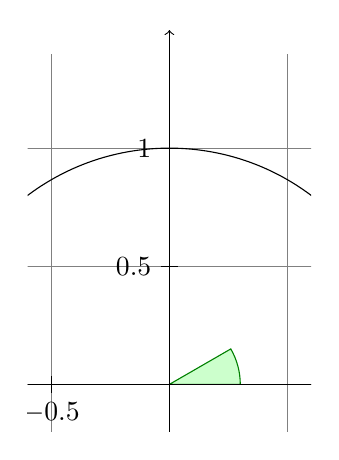
\begin{tikzpicture}[scale=3]
	\clip(-0.6,-0.2) rectangle (0.6,1.51);
	\draw[step=.5cm,help lines] (-1.4,-1.4)grid(1.4,1.4);
	\filldraw[fill=green!20,draw=green!50!black] 
	(0,0)-- (3mm,0mm)arc[start angle=0,end angle=30,radius=3mm]--cycle;
	\draw[->] (-1.5,0)-- (1.5,0);
	\draw[->] (0,-1.5)-- (0,1.5);
	\draw(0,0)circle[radius=1cm];
	
	\foreach\x in {-1,-0.5,1}
		\draw (\x cm,1pt)-- (\x cm,-1pt)node[anchor=north] {$\x$};
	\foreach \y in {-1,-0.5,0.5,1}
		\draw (1pt,\y cm)-- (-1pt,\y cm)node[anchor=east] {$\y$};
\end{tikzpicture}	
	
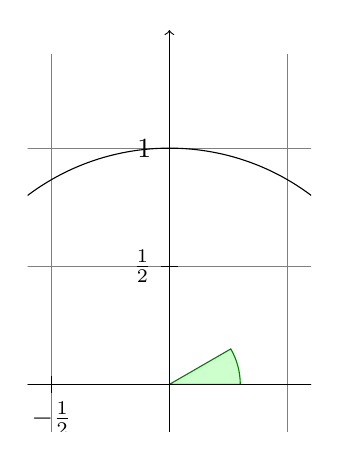
\begin{tikzpicture}[scale=3]
	\clip(-0.6,-0.2) rectangle (0.6,1.51);
	\draw[step=.5cm,help lines] (-1.4,-1.4)grid(1.4,1.4);
	\filldraw[fill=green!20,draw=green!50!black] 
	(0,0)-- (3mm,0mm)arc[start angle=0,end angle=30,radius=3mm]--cycle;
	\draw[->] (-1.5,0)-- (1.5,0);
	\draw[->] (0,-1.5)-- (0,1.5);
	\draw(0,0)circle[radius=1cm];
		
	\foreach \x/\xtext in {-1, -0.5/-\frac{1}{2}, 1}
		\draw (\x cm,1pt)-- (\x cm,-1pt) node[anchor=north] {$\xtext$};  
	\foreach \y/\ytext in {-1, -0.5/-\frac{1}{2}, 0.5/\frac{1}{2}, 1}
		\draw (1pt,\y cm)-- (-1pt,\y cm) node[anchor=east] {$\ytext$};
\end{tikzpicture}

